\documentclass{article}
\usepackage[round]{natbib}

\usepackage{fullpage}
\usepackage{amsmath}
\usepackage{amsfonts}
\usepackage{graphicx}
\usepackage{color}

\usepackage{setspace}

\usepackage{xr}
\externaldocument{supplement}

\DeclareMathOperator{\Var}{Var}

\newcommand{\aprcomment}[1]{{\textcolor{blue}{Comment: #1}}}
\newcommand{\E}{\mathbb{E}}

\title{Archaic introgression and the distribution
of shared functional variation under stabilizing selection}
\author{APR}
\date{\today}

\begin{document}
\maketitle    


\begin{abstract}
    .
\end{abstract}

\onehalfspacing

\section*{Introduction}

Genomic surveys of natural systems suggest that historical admixture among
diverged populations or closely related taxa commonly occurs
\citep{brandvain2014speciation,skoglund2015ancient,suvorov2022widespread} and
is potentially widespread in primate
\citep{tung2017contribution,sorensen2023genome} and hominin
\citep{wolf2018outstanding,peter2020100} evolution. Admixture may therefore be
an important driver of phenotypic and molecular variation and shape the genetic
basis of complex traits. In humans, archaic introgression involving
Neanderthals and Denisovans has attracted considerable attention, with efforts
to describe the historical processes leading to observed distributions of
introgressed DNA in present-day populations
\citep{prufer2014complete,villanea2019multiple,chen2020identifying} and its
contribution to quantitative traits
\citep{sankararaman2016combined,wei2023lingering}.

Once introduced through admixture, introgressed alleles may be selected for or
against. Some introgressed haplotypes were positively selected in modern humans
\citep{huerta2014altitude,racimo2017signatures,enard2018evidence,gower2021detecting},
possibly due to locally adaptive variation that provided fitness advantages as
humans encountered novel environments. Despite some cases of adaptive
introgression, introduced alleles were more likely to have been selected
against in modern humans \citep{harris2016genetic,juric2016strength}. Since
Neanderthal and Denisovan population sizes were relatively small for hundreds
of thousands of years, theory predicts they would have accumulated deleterious
variants at an increased rate. Introgressed haplotypes loaded with more
deleterious mutations would then have quickly been selected against after
admixture. Mapping the distribution of Neanderthal-introgressed haplotypes in
humans shows a reduction of Neanderthal-related ancestry in enhancers and
regulatory regions
\citep{petr2019limits,telis2020selection,yermakovich2023long}. These
``deserts'' of Neanderthal ancestry support the hypothesis that introgressed
functional alleles were selected against
\citep{sankararaman2014genomic,sankararaman2016combined}.

There is growing genetic evidence that early \emph{H. sapiens} reciprocally
contributed to Neanderthal genomes
\citep{kuhlwilm2016ancient,hubisz2020mapping,harris2023diverse}. This
human-to-Neanderthal introgression occured tens or hundreds of thousands of
years prior to Neanderthal introgression in humans during modern human global
dispersal around 60 ka. This is supported by ``near modern'' \emph{H. sapiens}
outside of African around 120--100ka or earlier
\citep{schwarcz1988esr,grun2005u,beyer2021climatic}, potentially overlapping
with Neanderthals and providing opportunities for early contacts. While
estimates of the genomic contribution of early \emph{H. sapiens} to
Neanderthals vary, around $6\%$ of later Neanderthal genomes may have been
contributed through introgression from humans to Neanderthals
\citep{harris2023diverse}. If \emph{H. sapiens}-related haplotypes carried
fewer deleterious alleles due to their larger long-term effective population
size, human-introgressed DNA would have been favored in Neanderthal genomes.
The replacement of Neanderthal mitochondrial and Y chromosomes by early human
haplotypes supports such a model of post-admixture selection in the Neanderthal
lineage \citep{posth2017deeply,petr2020evolutionary}.

Models for selection against introgressed alleles are often based on load
arguments (in particular, differences in the rate of accumulation of
unconditionally deleterious variation in populations of different sizes) or
hybrid incompatibilities \citep{muller1942isolating}. Such arguments, founded
in population genetics theory, rarely take into account selection operating on
phenotypic variation or the relationship between genetic and phenotypic
variation. Many phenotypic traits are thought to be under stabilizing selection
\citep{sanjak2018evidence,sella2019thinking}, including gene regulation
\citep{gilad2006natural,hodgins2015gene,price2022detecting}. Because some of
the strongest signals of selection against Neanderthal-introduced alleles are
in regulatory regions \citep{sankararaman2014genomic}, stabilizing selection on
quantitative traits is particularly relevant to the dynamics of functional
genetic variation after introgression.

Stabilizing selection acts to maintain the phenotypic distribution of a trait
near some optimum, which is achieved by reducing phenotypic variation
(Figure~\ref{fig:stab-sel}A). When the mean phenotype of the population is close
to the phenotypic optimum, classical models predict that alleles contributing
to such a trait are subject to underdominant selection, i.e., selection against
the minor allele at a locus \citep{robertson1956effect}. This has proven to be
a useful model for understanding genetic architectures of traits under
stabilizing selection in single-population settings
\citep[e.g.,][]{keightley1988quantitative, simons2018population,
hayward2022polygenic}.

\begin{figure}[tb!]
    \centering
    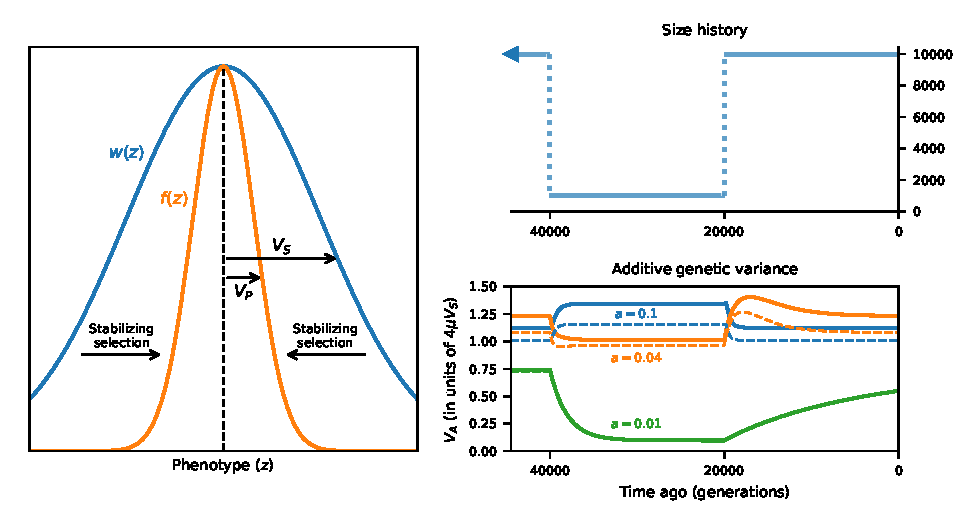
\includegraphics{../figures/one_pop.pdf}
    \caption{
        \textbf{Stabilizing selection and additive genetic variance in one population.}
        \aprcomment{See comparisons to simulations assuming free recombination in
        Figures~\ref{fig:one-popA}--\ref{fig:one-popC}.}
        \aprcomment{$w$ and $f$ need to match text}
        \aprcomment{Add the SHC model, and the ``vary SD'' fig as a panel here}
        \aprcomment{First figure should just be two left panels. Combine two
        right panels to figure 2.}
    }
    \label{fig:stab-sel}
\end{figure}

In diverged populations, genetic variation contributing to a trait under
stabilizing selection has a higher rate of turnover compared to neutrally
evolving loci \citep{yair2022population}. We might therefore expect an
accumulation of fixed differences in the \emph{H. sapiens} and Neanderthal
lineages at loci contributing to such a trait, even when the mean phenotype in
each population remains close to the same trait optimum. When a derived allele
at high frequency in one population is introduced to another population in
which is was previously absent, it will be at low frequency and subsequently
selected against. Likewise, if the ancestral allele is reintroduced to a
population fixed for a derived allele, the ancestral allele will be at low
frequency and will be selected against. In either case we should expect
selection against the introgressed allele, whether ancestral or derived and
regardless the historical relative sizes of the populations involved. This
prediction contrasts with the population-genetics ``load'' model, in which
haplotypes with fewer deleterious variants (such as those from the population
with larger historical size) are favored after introgression in either
direction.


\subsection*{Model}

We consider a polygenic trait for which an individual's (additive) genetic
value is the sum over all effects of alleles in their genome, so that for
individual $i$, \(G_i = \sum_l g_{l, i} a_l\), where $a_l$ is the effect size
of the derived allele at locus $l$, and \(g_{l,i}\in\{0,1,2\}\) is their
genotype at that locus (i.e., the number of alleles they carry at that locus).
With no linkage between trait-affecting loci, the expected additive genetic
variance is \(V_A = \sum_l 2p_l(1-p_l)a_l^2\), where $p_l$ is the allele
frequency at locus $l$. We ignore dominance and epistatic effects, so that
\(V_G = V_A\).  We further ingore environmental effects
\citep{simons2018population}, so that the phenotypic variance \(V_P=V_A\).

Stabilizing selection acts to reduce phenotypic variation around the optimum
value $O$ (typally set to zero), and we assume a Gaussian fitness function
(Figure~\ref{fig:stab-sel}A) so that relative fitness is given by \(f(G_i | O,
V_S) = \exp{(-(G_i - O)^2 / 2 V_S)}\). $V_S$ can be interpreted as the strength
of selection on the trait, where larger $V_S$ implies weaker selection. For a
population with mean phenotype at (or very close to) the optimum, the mean
fitness of the population (assuming a roughly normal distribution of phenotypic
values in the population) is \[\bar{w} \approx \int_{-\infty}^\infty f(G | 0,
V_S) \mathcal{N}(0, V_G) dG = \left(\frac{V_S}{V_S+V_G}\right)^{1/2}.\] Thus,
as the genetic variance increases, mean fitness among individuals in the
population decreases.

\subsubsection*{Mutation rates, effect sizes and genetic variance}

If all alleles contribute equally to the trait
(with effect sizes \(\pm a\) occurring in equal proportion),
\citet{keightley1988quantitative} showed that the dynamics of $V_G$ can be
approximated with the recursion
\[V_{G,t+1} \approx V_{G,t}\left(1-a^2/2(V_S+V_{G,t})\right)
\left(1-1/2N_e\right) + 2 \mu a^2,\]
where $\mu$ is the per-haploid, per-generation rate of mutation. In the
large-population-size limit, this gives the well-known result for
steady-state additive genetic variance,
\[V_G \approx 4\mu V_S,\] provided \(V_G \ll V_S\).

Mutations are not expected to each have the same effect size $a$, but rather
follow some distribution. Throughout, we assume effect sizes are drawn from a
normal distribution with mean 0 and given variance $V_M$. When population sizes
or effect sizes are small, drift dominates the dynamics of $V_G$, and at steady
state \citet{lande1976natural} found \[V_G \approx 4 N_e \mu V_M.\]
Interpolating between the selection- and drift-dominated regimes,
\begin{align}\label{eq:SHC}
    V_G & \approx \frac{4 \mu V_S}{1 + \frac{VS}{N_e V_M}}.
\end{align}
This, the ``stochastic
house-of-Cards'' (SHC) approximation (Figure~\ref{fig:stab-sel}B), was given by
\citet{burger1989much} and is discussed in detail in \citet[][Ch.
28]{walsh2018evolution}.

\subsubsection*{Approximating allelic dynamics via underdominance}

We model the distribution of allele frequencies underlying the trait using
the approximation that alleles are subject to symmetric underdominant
selection \citep{robertson1956effect,keightley1988quantitative}.
For an allele with (heterozygote) additive effect size $a$,
the selection coefficient
\[s\approx \frac{a^2}{2(V_S + V_G)} \approx \frac{a^2}{2V_S},\]
if $V_G \ll V_S$ \citep[e.g.,][]{simons2018population}. Allelic dynamics can
be modeled using the diffusion approximation, where the expected change
in mean allele frequency per generation is
\[\E[M_{\delta_p}] \approx -s p(1-p)(1-2p),\]
and the expected change in variance of the allele frequency per generation is
\[\E[V_{\delta_p}] \approx \frac{1}{4N_e}p(1-p).\]
%From this, because $s$ is always positive for any $a\not=0$, we see that
%selection pushes allele frequencies to zero if $p<1/2$ and to one if $p>1/2$.
%$p=1/2$ is an unstable equilibrium.

We extend the moments-based solution for the sample site-frequency spectrum
(SFS) \citep{jouganous2017inferring} to include underdominance with given
selection coefficient $s$ (\(=a^2/2(V_S+V_G)\)). The contribution of alleles
with effect size $a$ to the total genetic variance $V_G$ is then found by
computing the expected pairwise diversity from the SFS (with sample size $n$,
$\Phi_n$), as
\[V_{G,a} = 2a^2\sum_{j=1}^{n-1}\frac{j(n-j)}{n(n-1)}\Phi_n(j|a,\mu_a)da.\]
Here, $\mu_a$ is the mutation rate of alleles with effect size $a$. Then
assuming a normal distribution of effect sizes for new mutations, the total
genetic variance is
\[V_G=\int_{-\infty}^\infty V_{G,a}\mathcal{N}(0,V_M).\]

If $V_G$ is non-negligible compared to $V_S$, ignoring $V_G$ and using
$s=a^2/2V_S$ leads to lower estimates of additive genetic variance
(Figure~\ref{fig:toy-admixture}B). When mutation rates are large so that $V_G$
is not small compared to $V_S$, using $s=a^2/2(V_S+V_G)$ provides estimates of
$V_G$ that closely match simulations assuming free recombination between loci
(Figure~\ref{fig:toy-admixture}X,Y). Because $V_G$ can change over time, this
means that $s$ is no longer constant, but can change due to factors such as
non-constant demography that increase or reduce $V_G$.

\begin{figure}[tb!]
    \centering
    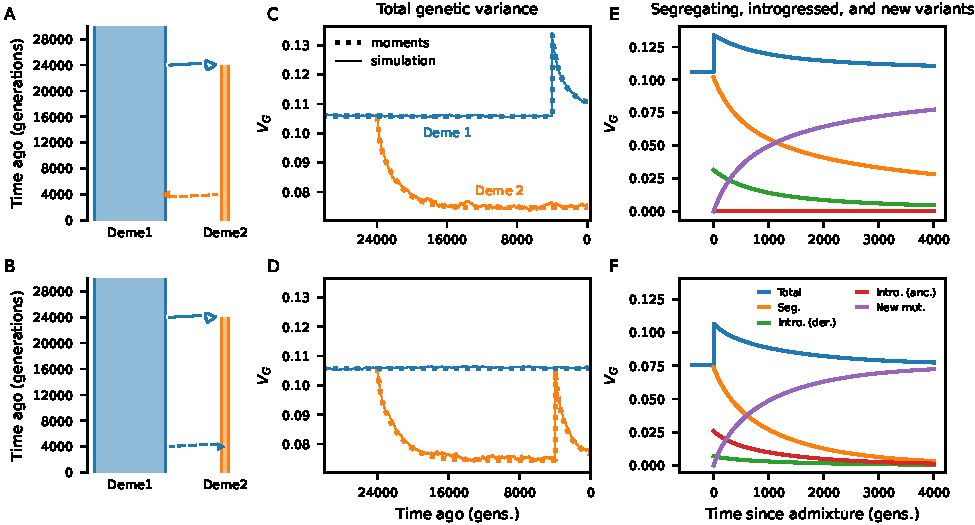
\includegraphics{../figures/reciprocal_admixture.pdf}
    \caption{
        \textbf{Predicting the genetic variance of a trait under stabilizing
        seletion and non-steady state demography.}
        \aprcomment{Make it in generations?}
        \aprcomment{Right two panels should go to supplement, move single-pop
        with size change from figure 1 to here.}
    }
    \label{fig:toy-admixture}
\end{figure}

\subsubsection*{Demographic history}

Our numerical solution for the SFS allows for non-constant population size
histories, population splits, continuous migration and admixture. Here, we
consider relatively simple scenarios involving population splits with
subsequent introgression events. We focus on parameter regimes relevant to
human-Neanderthal history. In a simple toy model -- which is not meant to
perfectly match any particular known or inferred history, but instead
demonstrate the effect of reciprocal introgression following population
divergence -- a population of size $N_e=10\,000$ splits into two, one remaining
size $10\,000$ and the other shrinking to size $1\,000$. They remain isolated
for $2N_e$ generations (or 500 thousand years, assuming an average generation
time of 25 years) and then introgression occurs from one branch to the other,
contributing $5\%$ ancestry to the recipient population
(Figure~\ref{fig:toy-admixture}X,Y).

The second model is meant to more closely resemble inferred human-Neanderthal
history, in which the ancestral population of size $N_e=10\,000$ splits into
the human and Neanderthal branches. At 250ka, an early human-to-Neanderthal
introgression contributes $5\%$ ancestry to Neanderthals. The human branch
shrinks to size $1\,000$ 60ka, followed by exponential growth to $20\,000$ at
present time. Neanderthals contribute $2\%$ ancestry to this bottlenecked and
expanding human population at 50ka, after which they go extinct
(Figure~\ref{fig:neand-to-human}A).

In each scenario, we track genetic diversity and phenotypic variance before and
after admixture to understand allele frequency and haplotype dynamics. The
trait optimum is kept at $0$ in all branches, so that no optimum shift occurs,
and the strength of selection $V_S=1$ remains constant.

\begin{figure}[t!]
    \centering
    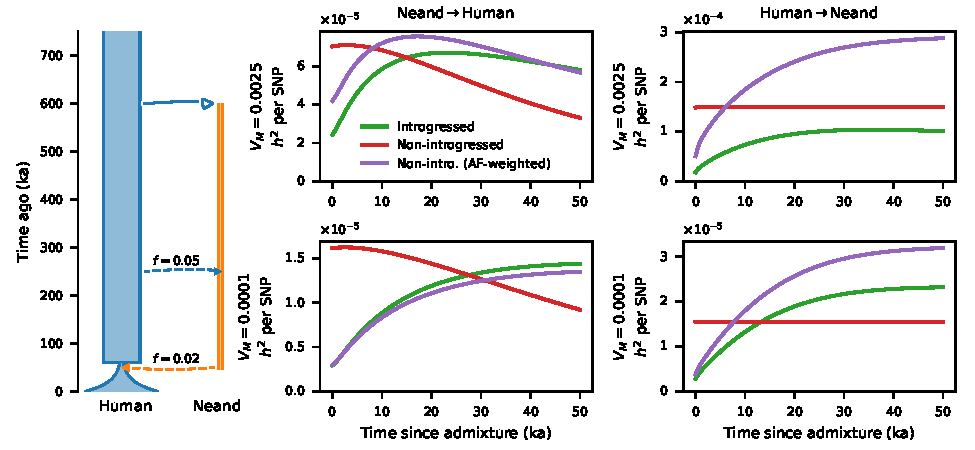
\includegraphics{../figures/neanderthal_admixture.pdf}
    \caption{
        \textbf{}
        \aprcomment{Show total/introgressed/non-introgressed in both directions
        with both $\sigma_M$.}
    }
    \label{fig:neand-to-human}
\end{figure}

\section*{Results}

\subsection*{Additive genetic variance after admixture}

We expect genetic variance to increase after introgression. The amount that
genetic variance increases depends on the allelic differences accumulated
between populations and the effects of those alleles. Assuming no linkage,
dominance or epistasis, \(V_G=\sum_l 2p_l(1-p_l)a_l^2\). After admixture, with
proportion $f$ contributed by the source population (labeled 0) into the focal
population (labeled 1), \(p_l = fp_{l,0} + (1-f)p_{l,1}\). Plugging into the
expression for $V_G$ and after some simple algebra (Appendix,
section~\ref{sec:VG-admixture}), we can express the expected genetic variance
directly after admixture as \[V_G = fV_{G,0} + (1-f) V_{G,1} + 2f(1-f)\sum_l
F_{2,l} a_l^2,\] where $F_2 = (p_0 - p_1)^2$ is the squared difference in
allele frequencies at a locus \citep{peter2016admixture}. This result is known
\citep[e.g.,][]{tufto2000quantitative}, showing that additive variance is equal
to that in the source populations weighted by their contributions, plus a term
that depends on the divergence at trait-affecting loci between the populations
weighted by the quadratic factor $2f(1-f)$.

$F_2$ at a given locus depends on the demographic history
relating the two populations and the effect size at the locus due to selection
on the trait. In the infinitesimal limit, involving many loci each of
vanishingly small effect, dynamics at a given locus will be approximately
neutral, so that $F_2$ depends only on the demography. In this case,
\begin{align}
    V_G & \approx f V_{G,0} + (1-f) V_{G,1} + 2f(1-f)\mathbb{E}[F_2] \sum_l a_l^2 \\
    \nonumber
    & = f V_{G,0} + (1-f) V_{G,1} + 2f(1-f)\mathbb{E}[F_2] L V_M,
\end{align}
where $L$ is the number of trait affecting loci.

\subsubsection*{Predicted $V_G$ from the SFS}

For $a \not\approx 0$, the assumption of neutral evolution will lead to
overestimates of $F_2$ compared to underdominant selection. We can compute
expected $V_G$ both before and after admixture using the diffusion
approximation for the joint SFS with underdominance. Comparing to simulations
with free recombination between loci (Appendix,
section~\ref{sec:VG-admixture}), we find that this provides an excellent fit to
average observed $V_G$ over time (Figure~\ref{fig:toy-admixture}C,D). In
general, admixture causes a sudden increase in $V_G$ followed by a fairly rapid
return to pre-admixture levels.

Modeling the dynamics of genetic variance using the SFS lets us examine
contributions to $V_G$ from different classes of mutations, such as those at
different frequencies or arising at different times, and how those
contributions change over time. Of interest is the contribution to $V_G$ from
alleles that were already segregating in the recipient population, those that
were introduced through introgression, and new mutations since the time of
admixture (Figure~\ref{fig:toy-admixture}). In many scenarios, the initial
divergence of the two populations will have occurred long enough before the
admixture event, so that the mutations underlying $V_G$ are largely unique in
each population. After mixing, previously segregating and introgressed alleles
go to fixation or loss, and the variance of the trait is increasingly due to
new mutations. 

Introgressed variation can initially make up a considerable portion of $V_G$,
with those alleles being either newly introduced derived alleles or
reintroduced ancestral alleles. The relative sizes of the two populations
impacts the number of each, as derived alleles will accumulate more readily in
a population with smaller effective size. Nonetheless, the increase in $V_G$
can be fairly similar in either direction of introgrssion, as the term
\(2f(1-f)\sum_l F_{2,l} a_l^2\) contributes in either case and can be much
larger than $f V_G$ from the source population.

\subsubsection*{Complex demography and partitioning heritability by origin of alleles}

We used a historical model more closely resembling inferred human-Neanderthal
history (Figure~\ref{fig:neand-to-human}A) to explore the effects of population
size changes and reciprocal admixture on the additive genetic architecture of
traits under stabilizing selection. As expected
(Figure~\ref{fig:toy-admixture}), population contractions decrease $V_G$ as the
increased rate of drift reduces allelic diversity at trait-affecting loci, and
introgression increases $V_G$ in both directions of gene flow.

Because the genetic architectures considered here are purely additive, we can
track mutations in an admixed populations by whether they were previously
segregating, fixed or lost in either parental populations or if they arose as
new mutations since the time of admixture (Methods Section X). This allows us
to partition $V_G$ by contributions from these different sets of mutations. At
low introgression proportions, as modeled here, the majority of $V_G$ is still
contributed by previously segregating, non-introgressed mutations (Figure XAB).
$V_G$ due to existing mutations decays monotonically over time and is fairly
rapidly replace by new mutations (Figure XCD).

The average contribution of introgressed vs. non-introgressed SNPs to $V_G$
(i.e., $h^2$ per SNP) can similarly by tracked over time. For the
human-Neanderthal-like demographic model and genetic architectures considered
here, the contribution per SNP of introgressed variants is initally lower than
that of non-introgressed variants. These contributions change over time,
depending on mutational variance (Figure YA vs B), as well as demography
(comparing the two directions of introgression, Figure YC D). When weighting
$h^2$ per SNP of introgressed SNPs by matching to allele frequencies of
non-introgressed variants (Methods), relative contributions depend sensitively
on evolutionary parameters and the time since admixture.

\aprcomment{In discussion, point out that this makes interpreting results, such
as \cite{wei2023lingering}, challenging.}

\begin{figure}[t!]
    \centering
    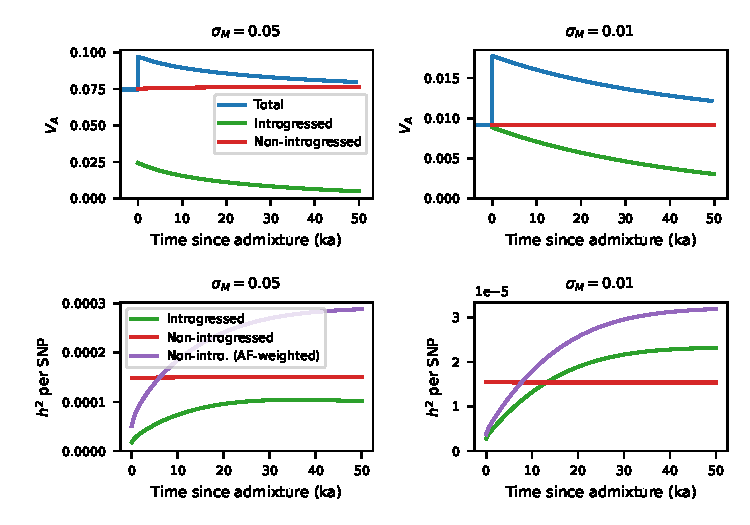
\includegraphics{../figures/human_admixture.pdf}
    \caption{
        \textbf{}
        \aprcomment{Put $h^2$ per SNP into its own figure.}
    }
    \label{fig:human-to-neand}
\end{figure}

\subsection*{The effects of linkage}

In the preceding sections, we find that approximating the dynamics of
trait-affecting alleles using an underdominance model
\citep{robertson1956effect} provides an excellent approximation of $V_G$ in
complex demographic scenarios. However, this relies on an absence of linkage
between trait-affecting alleles. The inclusion of linkage can lead to
noticeable effects on expected $V_G$, so that Equation~\ref{eq:SHC} slightly
overestimates $V_G$ at steady state
\citep{burger1989much,burger1994distribution,walsh2018evolution}.

To investigate the effects of linkage, we used chromosome-scale
individual-based simulations. By varying the mutation rate and the variance of
effect sizes of new mutations, we include scenarios ranging from low to high
polygenicity and from weak to strong selection on individual alleles. In this
and the following sections, we will highlight two effects of linkage. First,
we observe deviations of $V_G$ from expectations without linkage, which can be
large for highly polygenic traits. Second, selection on introgressed
trait-affecting alleles results in a reduction of introgressed ancestry in
surrounding regions.

With linkage between two or more alleles affecting a trait under stabilizing
selection, linkage disequilibrium (LD) can develop between alleles. Classicaly,
stabilizing selection will cause mutations of opposite-signed effects to be in
coupling LD and those of same-signed effects in repulsion LD
\citep{bulmer1971effect}. This has the effect of reducing $V_G$. For lower
mutational variances ($2N_e V_M\approx1$, Figure~\ref{fig:low_VM}), we observe
this phenomenon. With low mutational input, and thus low polygenicity, $V_G$ in
individual simulations closely matches expectations without linkage. As we
increase the mutation rate, $V_G$ is reduced relative to those expectations.
However, when the mutational variance is much larger ($2Ne V_m \approx 50$), we
see the reverse trend (Figure~\ref{fig:high_VM}). At low mutation rate, there
is a close match between observed $V_G$ and unlinked expectations, although
simulated values are slightly higher. As the mutation rate increases, $V_G$
increases to be relatively much larger that expectations, rather than smaller.

The strength of the deviation of $V_G$ between models with and without linkage
depends on a number of factors. The total mutation rate affects not only the
polygenicity, with higher mutation rates causing higher number of segregating
alleles, but also the mean recombination rate between those alleles, as they
will be more or less densely distributed in the genome. The distribution of
effect sizes plays an important role, as seen by the opposite trends in $V_G$
relative to unlinked predictions (Figure~X vs. Figure~Y), which are most
apparent with high mutation rates, and thus high polygenicity. In such cases,
there appear to be complex dynamics involving the Bulmer Effect
\citep{bulmer1971effect} and interference between selected alleles
\citep{hill1966effect}.

\subsubsection*{Introgressed ancestry is reduced around introduced
trait-affecting alleles}

Because introgressed trait-affecting alleles are selection against as the minor
allele, introgressed ancestry segments in the regions surrounding the selected
alleles will also be removed due to linkage. The expected reduction in such
introgressed ancestry will depend on the effect size of the trait-affecting
allele and the probability of recombination surrounding that locus. We first
consider a deterministic model of the dynamics of introgressed allele and
linked ancestry frequencies with variable recombination between them. This
simple model ignores the effects of drift and of interference between multiple
selected alleles.

We model a trait-affecting site with a fixed difference between the two
parental populations, in which the derived allele may be fixed in either
population. At the functional site, with admixture proportion $f$ from the
minor parental source, the initial frequency of the derived allele is either
$p_0=f$ or $p_0=1-f$. Over one generation, the expected allele frequency at the
selected locus is, to leading order in $s$,
\begin{align}\label{eq:system-p}
    p_{t+1} & = p_t - s p_t(1-p_t)(1-2p_t),
\end{align}
with
\(s=a^2/2V_S\). As discussed above, if \(p_0<1/2\), \(p_t\rightarrow0\), and if
\(p_0>1/2\), \(p_t\rightarrow1\) as \(t\rightarrow\infty\).

We consider a neutral locus separated from the selected locus by recombination
probability $r$. Initially, the expected frequency of linked introgressed
ancestry is \(q_0=f\), which changes over time due to linked selection on the
trait-affecting allele. Letting \(D=Cov(p,q)\) be the standard covariance
measure of LD between the two loci, $q$ is expected to change as
\begin{align}\label{eq:system-q}
    q_{t+1} & = q_t - s D_t(1-2p_t).
\end{align}
Initially, \(D_0=\pm f(1-f)\), with \(D\) being
positive if \(p_0=f\) and negative if \(p_0=1-f\). LD between the loci changes
deterministically over time, due to both selection and recombination, so that
\begin{align}\label{eq:system-D}
    D_{t+1} = D_t - r D_t - s D_t (1-2p_t)^2.
\end{align}
Together, this forms a
simple nonlinear system of equations for the deterministic change in allele
frequencies at the two loci and LD between them.

Using this model, we predict the changes in introgressed allele frequences and
LD after admixture for given effect size $a$ and recombination rate $r$
(Figure~\ref{fig:linkage-pred}). As expected, smaller effect sizes result in a
slower decay in introgressed ancestry frequency at both selected and linked
loci, and larger recombination rates more quickly decouple the linked ancestry
from the selected allele dynamics. Thus, the expected reduction in introgressed
ancestry is largest for larger effect sizes (Figure~\ref{fig:linkage-pred}X),
and LD between the selected and linked neutral alleles is largest for neutral
sites closest to the selected allele (Figure~\ref{fig:linkage-pred}Y).

We assessed the accuracy of the deterministic two-locus model using
individual-based forward-in-time simulations \citep{thornton2019polygenic}
under a simple demographic model (Figure~\ref{fig:toy-admixture}A), with
introgression fraction \(f=0.05\). We simulated a single chromosome of length 1
Morgan, with all mutations having effect sizes \(\pm a\) (\(a=0.02\) or
\(0.05\)), and we varied the total per-chromosome mutation rate (\(\mu=0.001\),
\(0.0025\) and \(0.01\)). For each fixed-difference mutation in the parental
populations, we determined the average introgressed ancestry surrounding such
loci (Methods).

The deterministic model (Equations~\ref{eq:system-p}--\ref{eq:system-D})
provides a very good approximation when mutation rates are small. As the
mutation rate increases in these simulations, polygenicity also increases so
that trait-affecting alleles are more densely distributed along the chromosome.
Deviations from the deterministic model are due to multiple selected alleles
affecting local introgressed ancestry. For the highest mutation rate shown
here, there are expected to be multiple other trait-affecting alleles within a
1 cM window around any focal SNP, which interact with each other and also
affect local ancestry proportions.

\begin{figure}[t!]
    \centering
    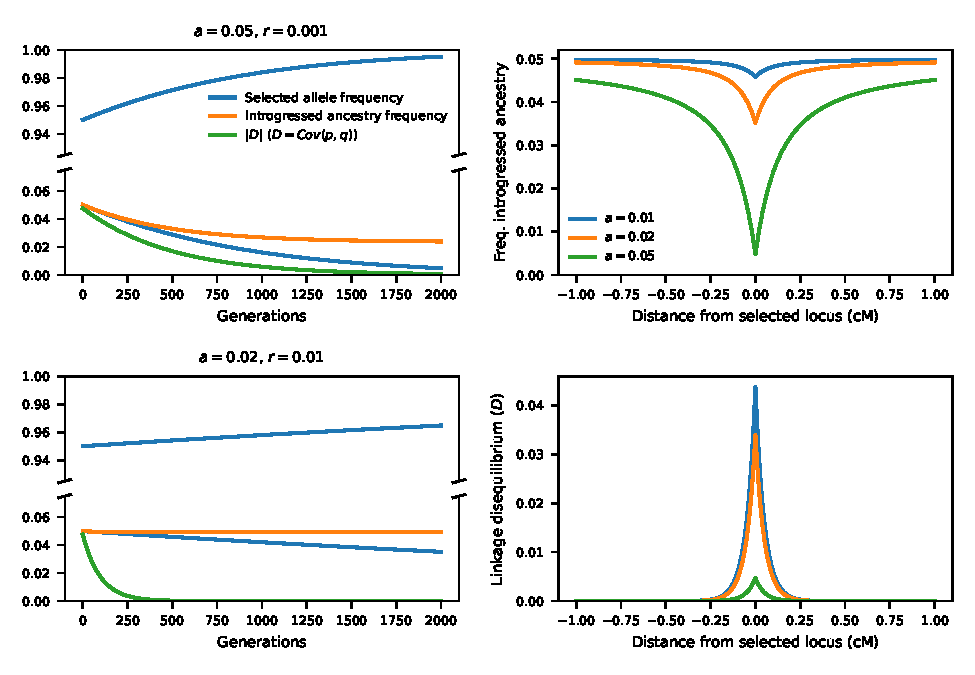
\includegraphics{../figures/linkage_predictions.pdf}
    \caption{
        \textbf{}
        \aprcomment{Linked allele frequency should always be minor, and labeled
        introgressed ancestry frequency}
        \aprcomment{Combine with next figure}
    }
    \label{fig:linkage-pred}
\end{figure}


\begin{figure}[t!]
    \centering
    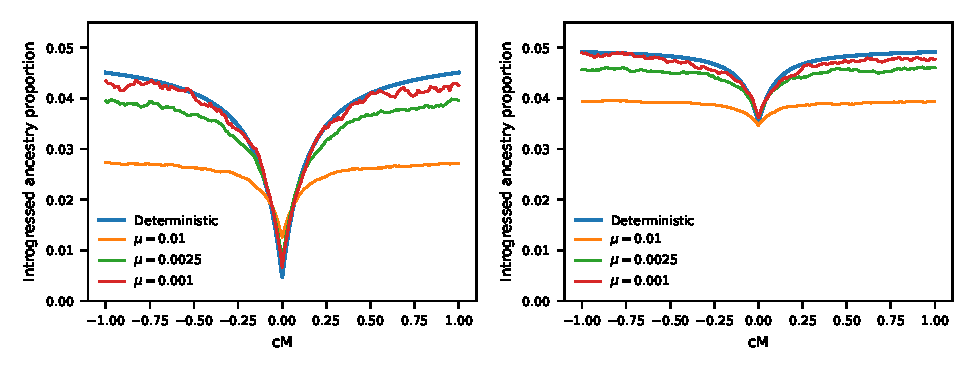
\includegraphics{../figures/linkage_simulation.pdf}
    \caption{
        \textbf{}
        \aprcomment{Combine with previous figure}
    }
    \label{fig:linkage-sim}
\end{figure}

\subsection*{Introgressed ancestry deserts are shared under stabilizing
selection and reciprocal introgression}

As shown in the previous section, introgressed ancestry is reduced around loci
with trait-affecting alleles regardless of the parental population the derived
allele is present in. We should therefore expect to observe reductions in
introgressed ancestry at the same trait-affecting loci after gene flow in
either direction. If introgression occurs in both directions, regions of
reduced introgressed ancestry will coincide around such loci, and introgression
``deserts'' that appear due to selection against trait-affecting alleles will
tend to be shared.

To demonstrate this effect, we performed chromosome-scale simulations under a
model of human-Neanderthal reciprocal introgression
\citep[Figure~\ref{fig:neand-to-human}A,][]{harris2023diverse}. Mutations
affecting a trait under stabilizing selection in each population could arise in
100 kb ``functional'' regions, spaced 1 Mb apart (Methods). Sampling
individuals from both the human and Neanderthal lineages, we observed the
average introgressed ancestry proportions were lowest within functional regions
and dipped in the surrounding regions (Figure~\ref{fig:deserts}A). This
corresponded to an increased proportion of ancestry deserts (defined as
    contiguous 50kb regions with no observed introgressed ancestry in the
sample) within and immediately surrounding the functional regions. Functional
regions also displayed an enrichment of \emph{shared} ancestry deserts, with
the probability of observing ancestry deserts (either within a population or
shared) decaying to background levels as the distance from the functional
region increases.

\begin{figure}[t!]
    \centering
    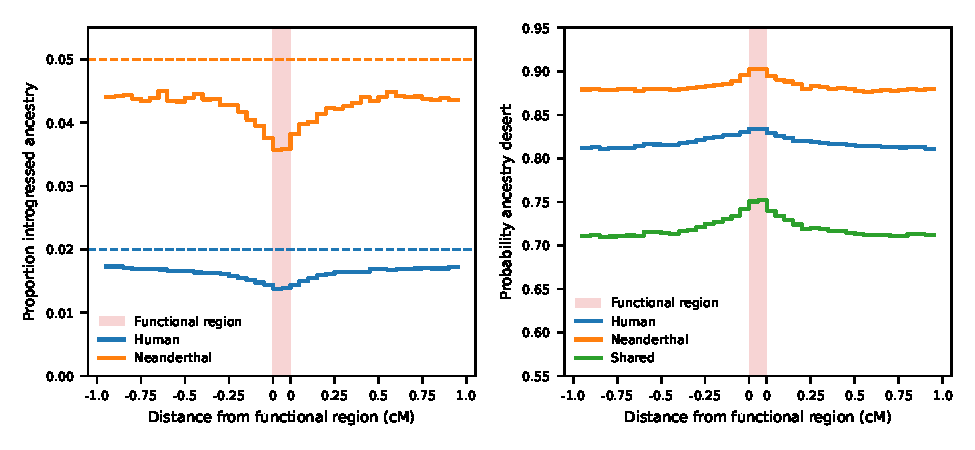
\includegraphics{../figures/introgression_deserts.SD_0.02.pdf}
    \caption{
        \textbf{}
    }
    \label{fig:deserts}
\end{figure}

\section*{Discussion}

\begin{itemize}
    \item Stabilizing selection with a constant optimum is an appropriate
        null model for the dynamics of trait variation and selection on
        alleles underlying those traits
    \item Stabilizing selection results in population genetic predictions
        for patterns of introgressed variation in and around functional
        regions that differ from both load- and incompatibility-based arguments
        \begin{itemize}
            \item Load-based models predict that haplotypes from the less ``loaded''
                population will be favored under introgression in either direction
                -- thus, regions of depleted ancestry after introgression in one
                direction will not be expected to also be introgressed ancestry
                deserts after admixture in the opposite direction
            \item \citet{mueller1942} originally pointed out that hybrid
                incompatibilities should not form at single loci -- classical
                incompatibilities require two or more loci, which are not
                expected to be tightly linked to one another. Thus, under a
                model of hybrid incompatibilities, the minor parent ancestry
                is again selected against, but those loci will be in different
                regions. Again, deserts are therefore not expected to overlap
                if selection is largely due to incompatibilities
            \item Instead, stabilizing selection causes introgressed DNA to be
                depleted at the same loci under bi-directional gene flow
                (could be thought of as single-locus incompatibility effects --
                but these are not incompatibilities in the classical sense,
                as the same effects occur even without admixture)
            \item A prediction we could make is that, if current models are correct
                that there has been introgression in both directions between
                \emph{H. sapiens} and Neanderthals, introgressed ancestry deserts
                should overlap with each other more often than expected by chance
            \item See Figure~\ref{fig:ancestry-deserts}
        \end{itemize}
    \item Shared deserts are most likely to form where moderate- or large-effect
        alleles have fixed in one population or the other -- this could provide
        an approach to map\dots?
    \item Selection in structured populations with ongoing migration or
        meta-populations -- SFS approach can handle this -- prospects for the
        future
    \item Some conjectures about hybrid zones
    \item Pleiotropy\dots!!!
\end{itemize}

\section*{Methods}

\subsection*{Computing expected genetic variance using the diffusion approximation}

\subsection*{Simulations with free recombination}

\subsection*{Individual-based simulations with linkage}

\bibliographystyle{genetics}
\bibliography{manuscript}

\appendix

\section{Additive genetic variance after admixture}\label{sec:VG-admixture}

\aprcomment{Start with ``Here we show that\dots''}

Suppose two population (labeled 0 and 1) diverged some time in the past and
then admix in proportions $f$ and $1-f$.

Assuming no linkage, dominance or epistasis (so \(V_G=V_A\)),
\[V_G = \sum_l 2p_l(1-p_l)a_l^2 = \sum_l \pi_l a_l^2,\]
where $\pi$ denotes expected pairwise diverisity.
At a given locus (dropping the $l$), after admixture the allele frequency is
\[p=f p_0 + (1-f) p_1,\]
so that
\begin{align*}
    2p(1-p) & = 2(f p_0 + (1-f) p_1)(1 - f p_0 - (1-f) p_1) \\
    & = f^2 2p_0(1-p0) + (1-f)^2 p_1(1-p1) + 2f(1-f) (p_0(1-p_1) + p_1(1-p_0)) \\
    & = f^2 \pi_{0,0} + (1-f)^2 \pi_{1,1} + 2f(1-f)\pi_{0,1}.
\end{align*}

Plugging in to the definition for $V_G$, we get after admixture
\[V_G = f^2 V_{G,0} + (1-f)^2 V_{G,1} + 2f(1-f)\sum_l \pi_{0,1,l}a_l^2.\]
We can write $\pi_{0,1}$ at a given locus in terms of $\pi_{0,0}$, $\pi_{1,1}$,
and $F_2(0,1)=(p_0-p_1)^2$ as \citep{peter2016admixture}
\[\pi_{0,1} = F_2(0,1) + \frac{1}{2}\pi_{0,0} + \frac{1}{2}\pi_{1,1}.\]
Then
\begin{align*}
    V_G & = f^2 V_{G,0} + (1-f)^2 V_{G,1} + 2f(1-f)\sum_l \left[F_{2,l}(0,1)
    + \frac{1}{2}\pi_{0,0} + \frac{1}{2}\pi_{1,1}\right] a_l^2 \\
    & = f^2 V_{G,0} + (1-f)^2 V_{G,1} + 2f(1-f)\left[\frac{1}{2}V_{G,0} 
    + \frac{1}{2}V_{G,1} + \sum_l F_{2,l}(0,1)a_l^2\right] \\
    & = \left(f^2 + f(1-f)\right) V_{G,0} + \left((1-f) + f(1-f)\right)V_{G,1}
    + 2f(1-f) \sum_l F_{2,i}(0,1)a_l^2 \\
    & = f V_{G,0} + (1-f)V_{G,1} + 2f(1-f)\sum_i F_{2,l}(0,1)a_l^2.
\end{align*}


\begin{figure}[tb!]
    \centering
    %\includegraphics{}
    \caption{
        \textbf{Dynamics of additive genetic variance in two populations with admixture.}
        Coupled with the equations for the decay of $V_G$ due to drift and selection,
        and the increase in $V_G$ through mutation, show that the expected dynamics
        are matched by simulations without linkage.
    }
    \label{fig:VG_dynamics}
\end{figure}

\section{Dynamics of introgressed alleles}

\section{Reciprocal depletion of functional variation}

While incompatibilities require two or more loci (Morgan, 1942), introgression
with stabilizing selection can create the appearance of a single-locus
incompatibility via underdominance\dots


\end{document}
